\documentclass[11pt, oneside]{article}   	% use "amsart" instead of "article" for AMSLaTeX format
\usepackage{geometry}                		% See geometry.pdf to learn the layout options. There are lots.
\usepackage{eurosym}
\geometry{letterpaper}                   		% ... or a4paper or a5paper or ... 
%\geometry{landscape}                		% Activate for for rotated page geometry
%\usepackage[parfill]{parskip}    		% Activate to begin paragraphs with an empty line rather than an indent
\usepackage{graphicx}				% Use pdf, png, jpg, or eps§ with pdflatex; use eps in DVI mode
								% TeX will automatically convert eps --> pdf in pdflatex		
\usepackage{amssymb}
\usepackage{amsmath}
\usepackage{systeme}
\usepackage{mathabx}
\usepackage{siunitx}
\usepackage{chemfig}
\usepackage{float}
\usepackage{tikz}
\usepackage{tkz-euclide}
\usetikzlibrary{angles,quotes}
\usepackage{subcaption}
\usepackage{afterpage}

\usepackage[section]{minted}
\renewcommand{\baselinestretch}{1.5}

\renewcommand{\MintedPygmentize}{/Users/estebancastillo/Library/Python/2.7/bin/pygmentize}

\renewcommand{\baselinestretch}{1.5}
\newcommand\blankpage{
    \null
    \thispagestyle{empty}
    \addtocounter{page}{-1}
    \newpage
    }

\title{\textbf{Aufgabe 5: Writer-Dokument}}
\author{Team-ID: 00000 \\ Team-Name: Name \\ Bearbeiter/-innen dieser Aufgabe: \\ Emilis Guzys \\ Leonard Kraus \\ C. V. Esteban}

\begin{document}

\textbf{}

\maketitle

\tableofcontents

\addcontentsline{toc}{section}{L\"osungsidee}
\section*{L\"osungsidee}
 \textbf{Am Anfang} denkt man direkt, dass es darum geht; einfach ein sogennantes \textit{"Sudoku"} zu l\"osen. Man m\"usste nur eine Menge $\pmb{L}$ (L\"osungsmenge) mit den folgenden Eigenschaften erstellen bzw. mithilfe einer logischen Maschine wie z.B. Prolog: 

\begin{equation*}
	\pmb{M}^{n \times 3} =
	\begin{pmatrix}
		1 & 3 & 5 \\
		2 & 4	 & 3 \\
		\ddots & \ddots & \ddots \\
		x_1a & x_2b & x_3c
	\end{pmatrix}
	\hspace{0.3cm} wobei \hspace{0.3cm}
	\forall x_ij: x_i \in [1 \hspace{0.1 cm} | \hspace{0.1cm} I]
\end{equation*}
\begin{equation*}
	\pmb{L} := \{(M_{1x}; M_{2y}; M_{3z} \dots M_{nr})/ M_{ab} \neq M_{cd}\}  \wedge	|\pmb{L}| = n \wedge  \pmb{L} \equiv \{1; 2; 3 ... n\}
\end{equation*}

Danach aber, nur nach den Beispieldatein angeschaut zu haben, scheint es komplizierter: Es kann ein oder mehrere Geschenke geben, die von keinem Kind gew\"unscht werden (\textit{wichteln2.txt}). Also, muss man das Problem ein bisschen erweitern und sich selber andere L\"osungswege denken. Aber eine Sache steht ganz klar: Man muss die \textbf{beste} Anordnung finden. Was passiert mit den Geschenken, die von niemandem gew\"unscht sind? Ich nehme an, dass man frei ist, sie zu irgendeinem Kind zugeben. Und da man weisst, dass \textit{jeder Kind ein Geschenk mitgebracht hat}; m\"ussen am Ende genauso viele Geschenke \"ubrig bleiben wie Kinder ohne Geschenke. \\
Die n\"achste wichtige Frage ganz genau zu beantworten ist: Was bedeutet dass eine Anordung besser als eine andere ist? In der Aufgabestellung steht dass die \textit{Parameter} nach den man eine L\"osung bewerten muss sind die Anzahl der Kinder, die sein erstes Wunsch bekommen haben; dann die die ihre zweite Wunsch bekommen haben und am Ende nat\"urlich die Anzahl der Kinder die sein Drittes Wunsch bekommen haben. Da wir die neue M\"oglichkeit betrachtet haben, dass ein Kind irgendein Geschenk bekommt; m\"ussen wir auch diese M\"oglichkeit ein Wert geben; und zwar in einer intuitiver Weise. Sobald es ein Kind mehr gibt, die sein erstes Wunsch bekommen hat; ist diese Anordnung besser. Egal ob deswegen, bekommen andere 3 Kinder z.B. ein zuf\"alliges Geschenk $\dots$ sehr pragmatish.
Mit diesen zwei Sachen sehr klar in Kopf (wie eine Anordnung besser als eine Anderer ist und, dass am Ende \textit{jedes} Geschenk wird zu \textit{einem} Kind zugeteilt) merkt man dass das Problem einfacher wird, indem man als Priorit\"at auf die W\"unsche passt. Egal was es f\}ur erste W\"unsche gibt, damit es keine andere bessere L\"osung gibt; muss man erst alle m\"ogliche erste-W\"unsche erf\"ullen. Aber man muss nicht davon ausgehen, dass es \textit{nur eine} Weise gibt, in der man \textit{alle m\"ogliche erste-W\"unsche} erf\"ullt. Genau daran liegt das wichtigste Teil der L\"osungsidee... keine F\"alle einfach h\"angen lassen. Wenn es mehrere Anordungen gibt, die diese Eigenschaft besitzen, dann folgt nat\"ulich die Frage ob es einer inzwischen den gibt, die besser als die anderen ist (ein Beispiel dazu in dem Beispiel Abteilung). Ganz grob kann man sagen dass wenn es 2 Kinder gibt, die als erster Wunsch das Geschenk 8 wollen; aber einer von den will das Geschenk 9 als zweite Wunsch und \textit{keiner anderer mehr}. Dann w\"are es besser das Geschenk 8 dem Kind geben, dessen zweite Wunsch nicht das Geschen 9 ist; damit man \textit{\"uberhaupt} das Geschenk 9 zu jemandem zuteilen k\"onnte. Jetzt wollen wir mit der richtigen Umsetzung anfangen.

\addcontentsline{toc}{section}{Umsetzung}
\section*{Umsetzung}
Jetzt geht es darum die oben erkl\"aerten Ideen als informatische Datensctrukturen und \textit{"Algorithmen"} zu \"ubersetzen. Dennoch das Quellcode wird nicht hier "erklaert", aber im "Quellcode" Abteilung. 
Wie es schon erw\"ahnt wurde, das Kern dieser L\"osung ist in einer sogennante logischen Maschine: Ein "State" wird gegeben (die m\"ogliche Kinder, die noch kein Geschenk bekommen haben bzw. ein Vektor/Kollektion dieser Form $-> [[k_i \hspace{0.2cm} [a \hspace{0.2cm} b \hspace{0.2cm} c]] \hspace{0.2cm} [k_j \hspace{0.2cm} [x \hspace{0.2cm} y \hspace{0.2cm} z]] \hspace{0.2cm}...\hspace{0.2cm}]$ wobei $k_i$ entspricht das Kinder Nummer, was dasselbe als das Index von $[a \hspace{0.2cm} b \hspace{0.2cm} c]$ ist). Dann, wie gesagt, guckt man nur auf die erste W\"unsche aller Kinder und stellt man eine andere Kollektion $-> [a \hspace{0.2cm} x \hspace{0.2cm} ...]$. Diese Kollektion ist sehr wichtig. Dadrin sind alle erste-W\"unsche und zwar so, dass z.B. $a$ auf der Position $0$ ist und entspicht das erstes Wunsch von dem ersten Kind... so haben wir kind und W\"unsche "verbinden". Am Ende machen wir aus dieser Kollektion ein sogennantes \textbf{Set}, so dass $[a \hspace{0.2cm} b \hspace{0.2cm} a \hspace{0.2cm} ...] -> \{a \hspace{0.2cm} b \hspace{0.2cm} ...\}$. Das machen wir um zu wissen, wie viele \textit{verschiedene} W\"unsche es gibt. Und jetzt das Punchline... diese letzte \textbf{Set} enth\"ahlt die maximale Anzahl von erste-W\"unsche (und auch genau welche) die erf\"ullt werden k\"onnten. Wir machen fast dasselbe mit die zweite-W\"unsche und dritte-W\"unsche. Die einzelne Unterschied liegt daran, dass wir die Geschenke nicht betrachten wollen, die als erstes Wunsch zugeteilt werden. Also, nochmal um die Idee deutlich klar zu machen: Es geht darum zu wissen, welche Geschenke \textbf{muss} ich als erstes-Wunsch zuteilen; welche als zweites Wunsch; und welche als drittes Wunsch. Deswegen ziehen wir von dem zweiten Set alle Geschenke aus dem ersten Set. Und beim n\"achstes mal (bei Set 3) ziehen wir alle Geschenke die in den anderen zwei Sets mitendrin sind.\\
Die n\"achste Idee ist die Agrupierung von Kinder die diesselbe erste-Wunsch bzw. zweite-Wunsch/drite-Wunsch haben. Das machen wir so: Wir definieren eine Abbildung (Funktion) $\Phi$ zwischen die Kollektion $[a \hspace{0.2cm} b \hspace{0.2cm} a \hspace{0.2cm} ...]$ und das Set $\{ a \hspace{0.2cm} b \hspace{0.2cm} ...\}$, sodass $\forall_x \in \pmb{S}: f(x) := \{(i_1; \hspace{0.2cm} i_2; \hspace{0.2cm} ...) \hspace{0.2cm} / \hspace{0.2cm} \pmb{K}[i_j] = x \}$ wobei $\pmb{K}[i_j]$ entspricht das element auf dem Index $i_j$ in der Kollektion $\pmb{K}$. Also, wir gucken uns an; welche Kinder gibt es, die dasselbe Geschenk als dasselbe Priorit"at wollen (erstes, zweites, drittes -Wunsch). Und das machen wir nochmal mit jedem Wunsch. "Wozu?" m\"ogen Sie fragen. Das Antwort wird sicherlich besser in der \textit{Beispiele} oder \textit{Quellcode} Abteilung erkl\"art werden. Aber das Antwort lautet ganz einfach dass wenn ich die Geschenke $[a \hspace{0.2cm} d \hspace{0.2cm} e]$ zu den Kinder $[x \hspace{0.2cm} y \hspace{0.2cm} z]$ gebe, w\"urde ich gerne wissen ob es irgendein Geschenk gibt, die \textbf{nur} von $[x \hspace{0.2cm} z]$ gewollt wurde. Wenn das so ist, dann weiss ich \textit{automatisch} dass dieses Geschenk $f$ ganz am Ende zuf\"allig zugeteilt wird. \\
In dieser Schritt kommt die logischen Maschine ins Spiel: Wir haben viele verschiedene m\"ogliche Anordungen und ein \textit{Parameter bzw. "Constraint"}, das die Suche regulieren k\"onnte. Dann lautet das Ziel bzw. \textit{Query} so: $\pmb{L} := \{ (l_1; \hspace{0.2cm} l_2 \hspace{0.2cm} ...) \hspace{0.2cm} / \hspace{0.2cm} l_i \in \Phi [i] \}$. Die optimalste L\"osung w\"are dass man $\pmb{L}$ bestimmen k\"onnte, sodass kein Geschenk, das als zweitens oder drittes Wunsch ist; sich "nach au{\ss}en r\"utschen m\"usste". Aber manchmal wird das einfach nicht m\"oglich. Deswegen, hat diese Query $\pmb{Q}_p$ ein Parameter $p$, die entspricht die maximale Anzahl von Geschenke die "sich r\"utschen d\"uerfen". Man fangt mit 0 an, und wenn es nicht klapp (wenn die Machine kein passendes $\pmb{L}$ findet), dann versucht man mit 1 und so weiter. Wenn alles gut l\"auft, dann kriegt man eine Kollektion von "kinder" bzw. Indexen. Die Zahlen die auf diesen Positionen sich befinden, sollten "gekreuzt" werden. Dieses Verfahren ist im Figur 1 deutlich zu erkennen.

\begin{figure} [h]
	\center
	\caption{Funktionelles Modell}
    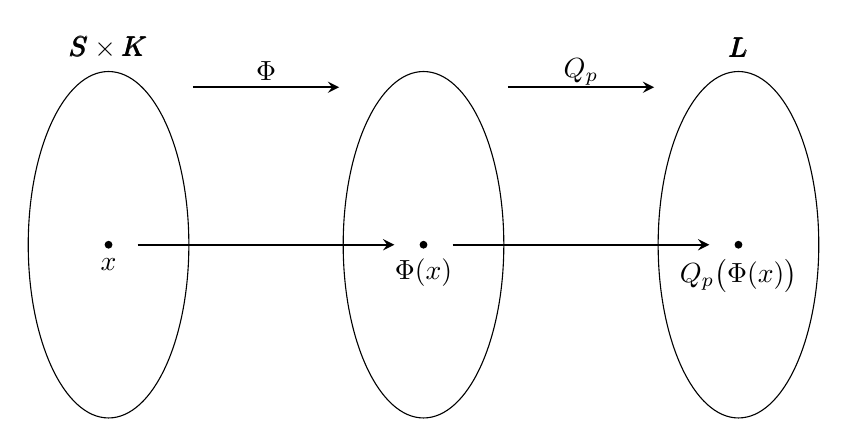
\begin{tikzpicture}[
    >=stealth,
    bullet/.style={
        fill=black,
        circle,
        minimum width=1pt,
        inner sep=1pt
    },
    projection/.style={
        ->,
        thick,
        shorten <=2pt,
        shorten >=2pt
    },
    every fit/.style={
        ellipse,
        draw,
        inner sep=0pt
    }
    ]
    \node at (2,4.7) {$\Phi$};
    \draw[projection] (1,4.5) -- (3,4.5);
    \node at (0,5) {$\pmb{S} \times \pmb{K}$};
    \node[bullet,label=below:$x$] (START)   at (0,2.5){};
    \node at (4,5) {$$};
    \node[bullet,label=below:$\Phi(x)$] at (4,2.5){};
    \node at (6,4.7) {$Q_p$};
    \draw[projection] (5,4.5) -- (7,4.5);
    \node at (8,5) {$\pmb{L}$};
    \node[bullet,label=below:$Q_p\big(\Phi(x)\big)$] (END) at (8,2.5){};
    
    \draw (0,2.5) ellipse (1.02cm and 2.2cm);
    \draw (4,2.5) ellipse (1.02cm and 2.2cm);
    \draw (8,2.5) ellipse (1.02cm and 2.2cm);

    \draw[projection] (0.3,2.5) -- (3.7,2.5);
    \draw[projection] (4.3,2.5) -- (7.7,2.5);
    \end{tikzpicture}
    \newline
\end{figure}

Man wiederholt das ganze mit kleinen ver\"anderungen, wie zum Beispiel dass beim zweiten mal muss man nicht auf dem ersten Wunsch passen, sonder auf dem dritten Wunsch. Aber im Grunde genommen ist das Verfahren dasselbe. Die Beispielen und das Quellcode werden alles besser bzw. genauer erkl\"aren.

\addcontentsline{toc}{section}{Beispiele}
\section*{Beispiele}
Als erstes Beispiel wird das L\"osungsprozess von \textit{Beispieldatei wichteln1.txt} ganz genau erk\"art. Erstmal lesen wir das \textit{.txt} Dokument und erstellen wir das folgende Struktur:

\begin{figure}[H]
	\begin{subfigure}{0.5\textwidth}
		\begin{align*}
 ([0 \hspace{0.2cm} (2 \hspace{0.2cm} 10 \hspace{0.2cm} 6)] & \\
    [1 \hspace{0.2cm} (2 \hspace{0.2cm} 7 \hspace{0.2cm} 3)] & \\
    [2 \hspace{0.2cm} (4 \hspace{0.2cm} 7 \hspace{0.2cm} 1)] & \\
    [3 \hspace{0.2cm} (3 \hspace{0.2cm} 4 \hspace{0.2cm} 9)] & \\
    [4 \hspace{0.2cm} (3 \hspace{0.2cm} 7 \hspace{0.2cm} 9)] & \\
    [5 \hspace{0.2cm} (4 \hspace{0.2cm} 3 \hspace{0.2cm} 2)] & \\
    [6 \hspace{0.2cm} (7 \hspace{0.2cm} 6 \hspace{0.2cm} 2)] & \\
    [7 \hspace{0.2cm} (10 \hspace{0.2cm} 2 \hspace{0.2cm} 4)] & \\
    [8 \hspace{0.2cm} (9 \hspace{0.2cm} 8 \hspace{0.2cm} 1)] & \\
    [9 \hspace{0.2cm} (4 \hspace{0.2cm} 9 \hspace{0.2cm} 6)]) 
\end{align*}
		\caption{Umgewandte Datenstruktur}
		\label{fig:subim1}
	\end{subfigure}
	\begin{subfigure}{0.5\textwidth}

		\begin{equation*}
			\pmb{M}^{10 \times 3}_0 =
			\begin{pmatrix}
				2 & 10 & 6 \\
				2 & 7	 & 3 \\
				4 & 7	 & 1 \\
				3 & 4	 & 9 \\
				3 & 7	 & 9 \\
				4 & 3	 & 2 \\
				7 & 6	 & 2 \\
				10 & 2 & 4 \\
				9 & 8	 & 1 \\
				4 & 9	 & 6 
			\end{pmatrix}
		\end{equation*}
		\hspace{0.2cm} \\
		\caption{Abstrakte Beschreibung}
	\end{subfigure}
	\caption{Anfangssituation}
	\label{fig:image2}
\end{figure}

An dieser Stelle m\"ussen wir die erste W\"unsche angucken und eine $\pmb{L}$\"osungsmenge daraus machen bzw. welche Geschenke zu welche Kinder als erstes Wunsch zugeteilt werden. An diesem Fall sieht es so aus (\textit{S} bedeutet Set und entspricht die Geschenke): 

\begin{equation*}
\begin{split}
\{S\{7 \hspace{0.2cm} 4 \hspace{0.2cm} 3 \hspace{0.2cm} 2 \hspace{0.2cm} 9 \hspace{0.2cm} 10\} \\
      (6 \hspace{0.2cm} 2 \hspace{0.2cm} 3 \hspace{0.2cm} 0 \hspace{0.2cm} 8 \hspace{0.2cm} 7)\}
\end{split}
\end{equation*}

Dann m\"usser wir aus $\pmb{M}^{10 \times 3}_0$ alle $\{(M_{i(1;2;3)}; M_{j(1; 2; 3)}; .../ (i;j; ...) \in \pmb{L}\}$ substrahieren um zu finden, welche Kinder noch keine Geschenk bekommen haben.

\begin{figure} [H]
	\begin{subfigure}{0.5\linewidth}
		\begin{align*}
			([1 \hspace{0.2cm} (2 \hspace{0.2cm} 7 \hspace{0.2cm} 3)]  \\
			 [4 \hspace{0.2cm} (3 \hspace{0.2cm} 7 \hspace{0.2cm} 9)]  \\
			 [5 \hspace{0.2cm} (4 \hspace{0.2cm} 3 \hspace{0.2cm} 2)]  \\
			 [9 \hspace{0.2cm} (4 \hspace{0.2cm} 9 \hspace{0.2cm} 6)])
		\end{align*}
	\end{subfigure}
	\begin{subfigure}{0.5\linewidth}
		\begin{equation*}
			\pmb{M}^{4 \times 3}_1 =
			\begin{pmatrix}
				2 & 7	 & 3 \\
				3 & 7	 & 9 \\
				4 & 3	 & 2 \\
				4 & 9	 & 6 
			\end{pmatrix}
		\end{equation*}
	\end{subfigure}
\end{figure}

Jetzt m\"ussen wir entscheiden, welche Geschenke \textit{als zweites Wunsch} zugeteilt werden. Aber in diesem Fall merkt man dass die Geschenke $7, 3$ und $9$ schon zugeteilt wurden und deswegen sollten wir in dieser Runde \textit{gar kein} Geschenk zuteilen... das ist genau das Antwort von dem Program:

\begin{equation*}
\begin{split}
\{S\{\}  \\
nil\}
\end{split}
\end{equation*}

Und selbsver\"andlich wenn man keine Geschenke zugeteilt hat, entspricht das Matrix $\pmb{M}^{4 \times 3}_1$ immer noch die Kinder die kein Geschenk bekommen haben. Also, brauchen wir kein weiteres Matrix zu presentieren. Dennoch jetzt werden die Geschenke definiert, die als drittes Wunsch zugeteilt werden:

\begin{equation*}
\begin{split}
\{S\{6\} \\
 (9)\}
\end{split}
\end{equation*}

Mit dem blo{\ss}en Augen h\"atte man auch merken k\"onnen, dass das einzige Geschenke, die \"ubrig geblieben ist, ist das Geschenk 6 und der einzelne Kind, das Kind an der Stelle 9 (\textit{Das Kind 0 existiert!}). Das letztes, das man noch machen muss; ist die Kinder und Geschenke definieren; die zu\"allig verbunden werden:

\begin{equation*}
\begin{split}
\{S\{1 \hspace{0.2cm} 5 \hspace{0.2cm} 8\}  \\
S\{1 \hspace{0.2cm} 4 \hspace{0.2cm} 5\}\}
\end{split}
\end{equation*}

Und das Antwort lautet:
\begin{center} \textbf{"The kids who receive their first wish are: $[6 \hspace{0.2cm} 2 \hspace{0.2cm} 3 \hspace{0.2cm} 0 \hspace{0.2cm} 8 \hspace{0.2cm} 7]$ those who receive their second wish are: $[]$ , and the ones receiving their third/last wish are $[9]$ And the kids $[1 \hspace{0.2cm} 4 \hspace{0.2cm} 5]$ will receive one random gift out of the following gifts $[1 \hspace{0.2cm} 5 \hspace{0.2cm} 8]$"} \end{center}

Als zweites Beispiel wird das Beispieldatei \textit{wichteln2.txt} pr\"asentiert. Aber diesmal ohne so viele Erkl\"arungen um Papier zu sparen.
 
\begin{figure}[H]
	\begin{subfigure}{0.5\textwidth}
		\begin{align*}
 ([0 \hspace{0.2cm} (4 \hspace{0.2cm} 6 \hspace{0.2cm} 5)] & \\
    [1 \hspace{0.2cm} (5 \hspace{0.2cm} 4 \hspace{0.2cm} 6)] & \\
    [2 \hspace{0.2cm} (6 \hspace{0.2cm} 4 \hspace{0.2cm} 5)] & \\
    [3 \hspace{0.2cm} (6 \hspace{0.2cm} 4 \hspace{0.2cm} 5)] & \\
    [4 \hspace{0.2cm} (5 \hspace{0.2cm} 4 \hspace{0.2cm} 6)] & \\
    [5 \hspace{0.2cm} (4 \hspace{0.2cm} 6 \hspace{0.2cm} 5)] & \\
    [6 \hspace{0.2cm} (4 \hspace{0.2cm} 5 \hspace{0.2cm} 6)] & \\
    [7 \hspace{0.2cm} (5 \hspace{0.2cm} 4 \hspace{0.2cm} 6)] & \\
    [8 \hspace{0.2cm} (6 \hspace{0.2cm} 5 \hspace{0.2cm} 4)] & \\
    [9 \hspace{0.2cm} (4 \hspace{0.2cm} 5 \hspace{0.2cm} 6)]) 
\end{align*}
		\caption{Umgewandte Datenstruktur}
		\label{fig:subim1}
	\end{subfigure}
	\begin{subfigure}{0.5\textwidth}

		\begin{equation*}
			\pmb{M}^{10 \times 3}_0 =
			\begin{pmatrix}
				4 & 6 & 5 \\
				5 & 4	 & 6 \\
				6 & 4 & 5 \\
				6 & 4	 & 5 \\
				5 & 4	 & 6 \\
				4 & 6	 & 5 \\
				4 & 5	 & 6 \\
				5 & 4 & 6 \\
				6 & 5	 & 4 \\
				4 & 5	 & 6 
			\end{pmatrix}
		\end{equation*}
		\hspace{0.2cm} \\
		\caption{Abstrakte Beschreibung}
	\end{subfigure}
	\caption{Anfangssituation}
	\label{fig:image2}
\end{figure}

Drei Kinder werden ausgew\"ahlt um ihre erstes Wunsch zu bekommen:

\begin{equation*}
\begin{split}
\{S\{4 \hspace{0.2cm} 6 \hspace{0.2cm} 5\} \\
(0 \hspace{0.2cm} 2 \hspace{0.2cm} 1)\}
\end{split}
\end{equation*}

Dann muss man die restliche Kinder \textit{erkennen}:

\begin{figure}[H]
	\begin{subfigure}{0.5\textwidth}
		\begin{align*}
 (  [3 \hspace{0.2cm} (6 \hspace{0.2cm} 4 \hspace{0.2cm} 5)] & \\
    [4 \hspace{0.2cm} (5 \hspace{0.2cm} 4 \hspace{0.2cm} 6)] & \\
    [5 \hspace{0.2cm} (4 \hspace{0.2cm} 6 \hspace{0.2cm} 5)] & \\
    [6 \hspace{0.2cm} (4 \hspace{0.2cm} 5 \hspace{0.2cm} 6)] & \\
    [7 \hspace{0.2cm} (5 \hspace{0.2cm} 4 \hspace{0.2cm} 6)] & \\
    [8 \hspace{0.2cm} (6 \hspace{0.2cm} 5 \hspace{0.2cm} 4)] & \\
    [9 \hspace{0.2cm} (4 \hspace{0.2cm} 5 \hspace{0.2cm} 6)]) 
\end{align*}
		\label{fig:subim1}
	\end{subfigure}
	\begin{subfigure}{0.5\textwidth}

		\begin{equation*}
			\pmb{M}^{7 \times 3}_1 =
			\begin{pmatrix}
				6 & 4	 & 5 \\
				5 & 4	 & 6 \\
				4 & 6	 & 5 \\
				4 & 5	 & 6 \\
				5 & 4 & 6 \\
				6 & 5	 & 4 \\
				4 & 5	 & 6 
			\end{pmatrix}
		\end{equation*}
		\hspace{0.2cm} \\
	\end{subfigure}
	\label{fig:image2}
\end{figure}

Jetzt muss man merken, dass kein anderes Kind irgendein Wunsch kriegen k\"onnte, weil alle gew\"unschte Geschenke schon zugeteilt wurden. Also, m\"ussen wir tats\"achlich kein Geschenk zuteilen:

\begin{equation*}
\begin{split}
\{S\{\}  \\
nil\}
\end{split}
\end{equation*}

Deswegen arbeiten wir mit dem Matrix $\pmb{M}^{7 \times 3}_1$ weiter. Und jetzt fragen wir nach den dritte W\"unsche. Nochmal ist einfach zu merken, dass kein drittes Wunsch erf\"ullt werden k\"onnte. Also, wir m\"ussen kein Geschenk zuteilen:

\begin{equation*}
\begin{split}
\{S\{\}  \\
nil\}
\end{split}
\end{equation*}

Da wir \textit{nur} $3$ Geschenke zu $3$ Kinder zugeteilt haben; sollten es $7$ Kinder und auch $7$ Geschenke \"ubrig bleiben:

\begin{equation*}
\begin{split}
\{S\{7 \hspace{0.2cm} 1 \hspace{0.2cm} 3 \hspace{0.2cm} 2 \hspace{0.2cm} 9 \hspace{0.2cm} 10 \hspace{0.2cm} 8\}  \\
S\{7 \hspace{0.2cm} 4 \hspace{0.2cm} 6 \hspace{0.2cm} 3 \hspace{0.2cm} 9 \hspace{0.2cm} 5 \hspace{0.2cm} 8\}\}
\end{split}
\end{equation*}

Deswegen, lautet das Antwort:

 \begin{center}\textbf{"The kids who receive their first wish are: $[0 \hspace{0.2cm} 2 \hspace{0.2cm}1]$,those who receive their second wish are: $[]$, and the ones receiving their third/last wish are $[]$ And the kids $[7 \hspace{0.2cm} 4 \hspace{0.2cm} 6 \hspace{0.2cm} 3 \hspace{0.2cm} 9 \hspace{0.2cm} 5 \hspace{0.2cm} 8]$ will receive one random gift out of the following gifts $[7 \hspace{0.2cm} 1 \hspace{0.2cm} 3 \hspace{0.2cm} 2 \hspace{0.2cm} 9 \hspace{0.2cm} 10 \hspace{0.2cm} 8]$"}\end{center}

\textbf{* Als Anmerkung} wollte ich auch sagen, dass \textit{logic programming} und Ich Grenzen haben. Beispieldateien wie \textit{wichteln7.txt} bieten ungeheuer viele M\"oglichkeiten, die von der logischen Engine \"uberpr\"uft werden m\"ussen damit die hier erkl\"arte L\"osung funktioniert. Das macht die Laufzeit des Programm gar nicht optimal und das Programm selbst keine optimale L\"osung f\"ur das verallgemeinertes Problem. Diese Grenzen zu \"uberbinden hoffen wir als Team in der kommende Zeit zu schaffen.

\addcontentsline{toc}{section}{Quellcode}
\section*{Quellcode}
Das Quellcode wird genauso wie bei der Umsetzung Abteilung beschrieben im Sinne Aussichtspunkt: Die wichtigsten Funktionen.
Die erste Funktion ist \textbf{description}, was bisher keine Name zugegeben wurde, weil die eigentlich eine Mittelfunktion bzw. Hilfsfunktion ist. Mithilfe von \textit{high-order-functions} ergibt diese Funktion ein \textit{Hashmap} wieder. In \textit{first-wish} sind alle Geschenke die als erstes Wunsch zugeteilt werden \textbf{m\"ussen}. Dasselbe passiert mit \textit{second-wish} und \textit{third-wish}. Damit sind wir im Raum $\pmb{S \times K}$.

\begin{minted}{clj}
(defn description
  [data]
  (let [per-column (map (fn [f]
                          (map (fn [v] [(first v) (f (second v))])
                               data))
                        [first second last])
        uniques (map (fn [v] (set (map second v))) per-column)
        first-wish (first uniques)
        second-wish (set/difference (second uniques) (first uniques))
        third-wish   (set/difference (last uniques) (set/union (second uniques)
                                                               (first uniques)))]
    {:per-column per-column :f first-wish :s second-wish  :l third-wish}))
\end{minted}

Jetzt kommt die Funktion $\Phi$. Diesmal wurde ein \textit{Threading Macro $(->>)$} und andere \textit{high-order-functions} wie \textit{filter} benutzt. Aus dieser Funktion kriegen wir welche Kinder wollen welche Geschenke als erstes-, zweitens-, und drittens- Wunsch.

\begin{minted}{clj}
(defn structure
  [data]
  (let [r (map (fn [f k]
                 (apply conj (map (fn [v] {v (->> (f (:per-column (description data)))
                                                  (filter #(= (second %1) v))
                                                  (map first))})
                                  (k (description data)))))
               [first second last] [:f :s :l])]
    (map #(if (empty? %1) {} %1) r)))
\end{minted}

Die Funktion \textbf{find-configuration} ist die logische Maschine (clojure.core.logic) die von David Nolen implementiert wurde. Die Ideen stammen aus Prolog; genauer gesagt aus Minikaren (eine minimalistische Implementation von \textit{constraint programming}). Und die Regeln, die ich definiert habe sind folgende: Ich w\"ahle $n$ Elemente aus $n$ Listen ( (rec-membero vars pool)), sodass wenn ich die Potenzmenge dieser Menge/Kollektion mir angucke; sollte kein Element dadrin sein, das ist auch bei $cond1$ oder $cond2$. Also, ich will die Indexes so ausw\"ahlen, dass es kein anderes Geschenk die genau nur auf den Indexen stehen kann.

\begin{minted}{clj}
(defn find-configuration
  [parameter pool cond1 cond2]
  (if (empty? pool)
    '()
    (let [vars (repeatedly (count pool) logic/lvar) 
          S (map #(remove (fn [_] (= _ nil)) %1) (Superset [] vars))]  
      (logic/run 1 [q]

        (rec-membero vars pool) 

        (macro/symbol-macrolet [a (count (filter (fn [c] (membero-coll c S)) cond1))
                                b (count (filter (fn [c] (membero-coll c S)) cond2))]
                               (fd/eq
                                (<= a parameter)
                                (<= b parameter))) 
        
        (logic/== q vars)))))
\end{minted}

Am Ende mache ich ein \textit{Tester} um zu \"uberpr\"ufen ob alles in Ordnung gelaufen ist. Alles ist gut, wenn am Ende die erste-, zweite-, dritte- W\"unsche und die sogennante \textit{free-spots} zu der gesamten Anzahl der Kinder addieren (dasselbe passiert mit den Geschenken).

\begin{minted}{clj}
(defn true-test []
  (let [answer (map (fn [f]
                      (apply set/union (map (fn [c]
                                              (f (first c)))
                                            [first-column-pairing
                                             second-column-pairing
                                             third-column-pairing
                                             free-spots])))
                    [first second])]
    (= (count (first answer)) (count (second answer)))))
\end{minted}

Da ich die Dateien aus einem .txt File gelesen habe, sollte ich auch das Antwort auf demselben File schreiben. Das Antwort ist ein gr{\ss}er String, das aus verschiedenen Teilen besteht: Erst sind die Kinder, die sein erstes Wunsch bekommen und so und so fort.

\begin{minted}{clj}
(defn answer-paolo []
  (let [output (if (true-test)
                 (str "\n The kids who receive their first wish are: "
                      (into [] (first (vals first-column-pairing))) "\n"
                      ",those who receive their second wish are: "
                      (into [] (first (vals second-column-pairing))) "\n"
                      ", and the ones receiving their third/last wish are "
                      (into [] (first (vals third-column-pairing)))

                      (if (empty? (first (vals free-spots)))
                        ""
                        (str "\n And the kids "
                             (into [] (first (vals free-spots)))
                             " will receive one andom gift out of the following gifts "
                             (into [] (first (keys free-spots))))))
                 "Something went wrong")]
    (with-open [wrtr (clojure.java.io/writer
                      (io/resource "clojure_version/aufgabe5sample3.txt")
                      :append true)]
      (.write wrtr output))
    output))
\end{minted}        

\textbf{Das ganzes Quellcode } kann man unter das GitHub Repository \textit{BundeswettbewerbInformatik} von dem User \textit{steve0el0crack} finden.

\end{document}